\documentclass{article}
\usepackage[utf8]{inputenc}
\usepackage{listings} % needed for the inclusion of source code

\title{Wavelet Analysis}
\author{Mgr. Patrik Pekarčík}
\date{March 2019}

\usepackage{natbib}
\usepackage{graphicx}
\lstset{numbers=left, numberstyle=\tiny, stepnumber=1, numbersep=5pt, frame=single, breaklines=true, language=bash}

\begin{document}

\maketitle

\section{Introduction}
Wavelets are mathematical functions that cut up data into different frequency components, and then study each component with a resolution matched to its scale. 
They have advantages over traditional Fourier methods in analyzing physical situations where the signal contains discontinuities and sharp spikes. 
Wavelets were developed independently in the fields of mathematics, quantum physics, electrical engineering, and seismic geology. 
Interchanges between these fields during the last ten years have led to many new wavelet applications such as image compression, turbulence, human vision, radar, and earthquake prediction. \citep{graps1995introduction}

\section{Wavelet basics}
The wavelet analysis procedure is to adopt a wavelet prototype function, called an analyzing wavelet or mother wavelet.
Temporal analysis is performed with a contracted, high-frequency version of the prototype wavelet, while frequency analysis is performed with a dilated, low-frequency version of the same wavelet. 
Because the original signal or function can be represented in terms of a wavelet expansion (using coefficients in a linear combination of the wavelet functions), data operations can be performed using just the corresponding wavelet coefficients. 
And if you further choose the best wavelets adapted to your data, or truncate the coefficients below a threshold, your data is sparsely represented. 
This sparse coding makes wavelets an excellent tool in the field of data compression.

Wavelet transforms comprise an infinite set. The different wavelet families make different trade-offs
between how compactly the basis functions are localized in space and how smooth they are.
Some of the wavelet bases have fractal structure. The Daubechies wavelet family is one example (see Figure \ref{fig:daubechies})

\begin{figure}[h!]
\centering
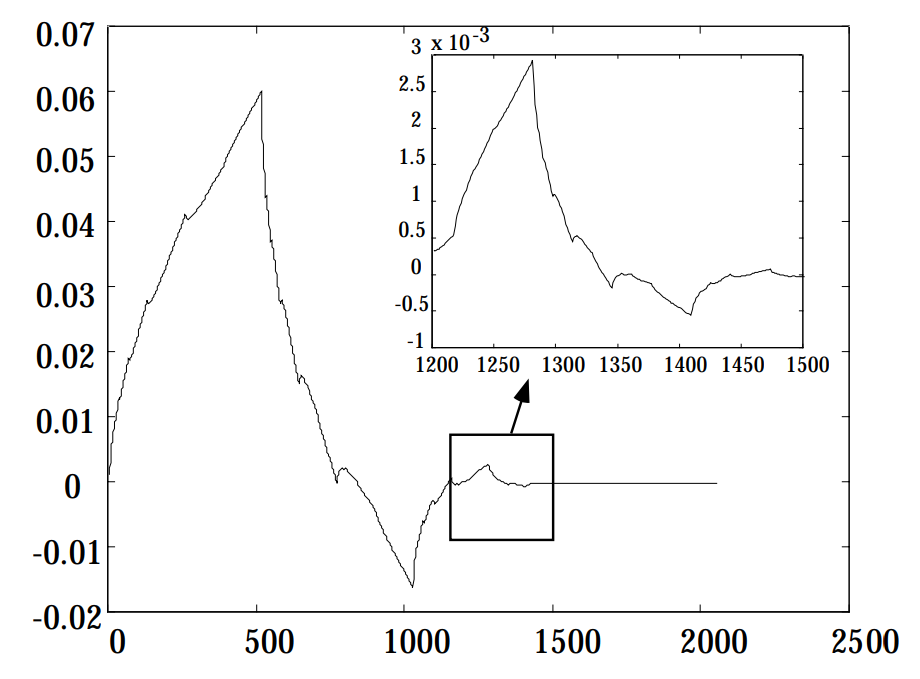
\includegraphics[scale=0.45]{daubechies.png}
\caption{\textbf{The fractal self-similiarity of the Daubechies mother wavelet.} This figure was generated using the WaveLab command: \(>wave=MakeWavelet(2,-4,‘Daubechies’,4,‘Mother’,2048)\). The inset figure was created by zooming into the region x=1200 to 1500.}
\label{fig:daubechies}
\end{figure}

Within each family of wavelets (such as the Daubechies family) are wavelet subclasses distinguished by the number of coefficients and by the level of iteration. 
Wavelets are classified within a family most often by the number of vanishing moments. 
This is an extra set of mathematical relationships for the coefficients that must be satisfied, and is directly related to the number of coefficients (1). 
For example, within the Coiflet wavelet family are Coiflets with two vanishing moments, and Coiflets with three vanishing moments.

Now we begin our tour of wavelet theory, when we analyze our signal in time for its frequency
content. Unlike Fourier analysis, in which we analyze signals using sines and cosines, now we use
wavelet functions.

\subsection{THE DISCRETE WAVELET TRANSFORM}

Dilations and translations of the “Mother function,” or “analyzing wavelet” \(\Phi(x)\), define an orthogonal basis, our wavelet basis:

\begin{equation}
\Phi_{(s,l)} (x) = 2^{-\frac{s}{2}} \Phi(2^{-s} x-l)
\label{eq:mother-function}
\end{equation}

The variables $s$ and $l$ are integers that scale and dilate the mother function $\Phi$ to generate
wavelets, such as a Daubechies wavelet family. The scale index $s$ indicates the wavelet’s width, and
the location index $l$ gives its position. Notice that the mother functions are rescaled, or “dilated”
by powers of two, and translated by integers. What makes wavelet bases especially interesting is
the self-similarity caused by the scales and dilations. Once we know about the mother functions, we
know everything about the basis.

To span our data domain at different resolutions, the analyzing wavelet is used in a scaling
equation:

\begin{equation}
W(x) = \sum_{k=-1}^{N - 2} (-1)^{k}c_{k+1}\Phi(2x + k)
\label{eq:scaling-equation}
\end{equation}

where $W(x)$ is the scaling function for the mother function $\Phi$, and $c_k$ are \textbf{the wavelet coefficients}.
The wavelet coefficients must satisfy linear and quadratic constraints of the form

\begin{equation}
\sum_{k=0}^{N-1} c_k = 2,\ \ \ \sum_{k=0}^{N-1} c_k c_{k+2l} = 2\delta_{l,0}
\label{eq:wavelet-coefficients}
\end{equation}

where $\delta$ is the delta function and $l$ is the location index.

One of the most useful features of wavelets is the ease with which a scientist can choose the
defining coefficients for a given wavelet system to be adapted for a given problem. In Daubechies’
original paper \cite{daubechies1988orthonormal}, she developed specific families of wavelet systems that were very good for representing polynomial behavior. The Haar wavelet is even simpler, and it is often used for educational
purposes.

It is helpful to think of the coefficients $\{c_0,...,c_n\}$ as a filter. The filter or coefficients are placed
in a transformation matrix, which is applied to a raw data vector. The coefficients are ordered using
two dominant patterns, one that works as a smoothing filter (like a moving average), and one pattern
that works to bring out the data’s “detail” information. These two orderings of the coefficients are
called a quadrature mirror filter pair in signal processing parlance.

\subsection{Commented Wavelet calculation in R-lang}

For better understanding of Discrete Wavelet Transform we will discuss some codeline in R-lang showing, whas is happening.
In this example we will be using R-lang library called \texttt{waveslim} \cite{brandonwhitcher2019}, whitch supports many wavelet mother functions (haar, d4, mb4, w4, bs3.1, fk4, d6, fk6, d8, fk8, la8, mb8, bl14, fk14, d16, la16, mb16, la20, bl20, fk22, mb24).

\begin{figure}[h!]
\begin{lstlisting}
install.packages("waveslim")
library(waveslim)
\end{lstlisting}
\caption{Library installation and loading.}
\label{code:library}
\end{figure}

After including library we should prepare some signal which will be processed later. Firstly i will prepare simple signal with one peak.

\pagebreak

\begin{figure}[h!]
\begin{lstlisting}
x = 1:1024
yy = ifelse(x <= 100, 0, ifelse(x < 102, 1, 0))
\end{lstlisting}
\caption{Preparing sample signal.}
\label{code:samples}
\end{figure}

\begin{figure}[h!]
\centering
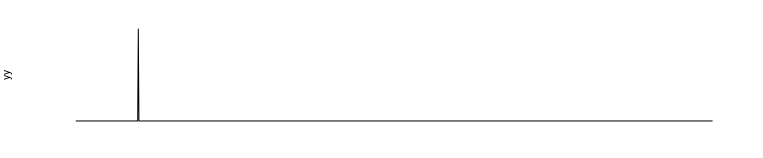
\includegraphics[scale=0.55]{basic-signal.png}
\caption{Prepared signal ploted with code \texttt{plot(yy, type = "l", axes = FALSE, mmain = "Data signal")}.}
\label{fig:sample-signal}
\end{figure}

In selected library calculation of Discrete Wavelet Transform is simple, because of calling one function called \texttt{dwt}. This function is very powerfull thanks to it's parameters. In parameters we can select whitch wavelet mother function it will be using, and we can select how many levels it will calculate for smoothing signal. Next we are showing example of Daubechies wavelet presented in previous section of 4 levels.


\begin{figure}[h!]
\begin{lstlisting}
dwtoutput <- dwt(yy, wf="d4", n.levels=4, boundary="periodic")
# Adding human readable names to signals
names(dwtoutput) <- c("level 1", "level 2", "level 3", "level 4", "smoothed")
\end{lstlisting}
\caption{Calculation of Daubechies signal smoothing.}
\label{code:dwt}
\end{figure}

Here we smoothed signal \texttt{yy} and now we are going to discover what is in output of this call (write \texttt{dwtoutput} in r console and watch the output). Firstly we can see that all levels are present in output. For better understanding of vectors next codelines will present them in plots.

\pagebreak

\begin{figure}[h!]
\begin{lstlisting}
# plot default data
par(mfcol=c(6,1), pty="m", mar=c(5-2,4,4-2,2))
plot.ts(yy, axes=FALSE, ylab="", main="Calculating wavelet from specified (yy) signal")

# plot 4 steps of dwt transforms
for(i in 1:4)
  plot.ts(up.sample(dwtoutput[[i]], 2^i), type="h", axes=FALSE,
          ylab=names(dwtoutput)[i])

# plot transformed signal
plot.ts(up.sample(dwtoutput$smoothed, 2^4), type="h", axes=FALSE,
        ylab=names(dwtoutput)[5])


\end{lstlisting}
\caption{Plotting whole output of \texttt{dwt} calculation.}
\label{code:plotting}
\end{figure}

\begin{figure}[h!]
\centering
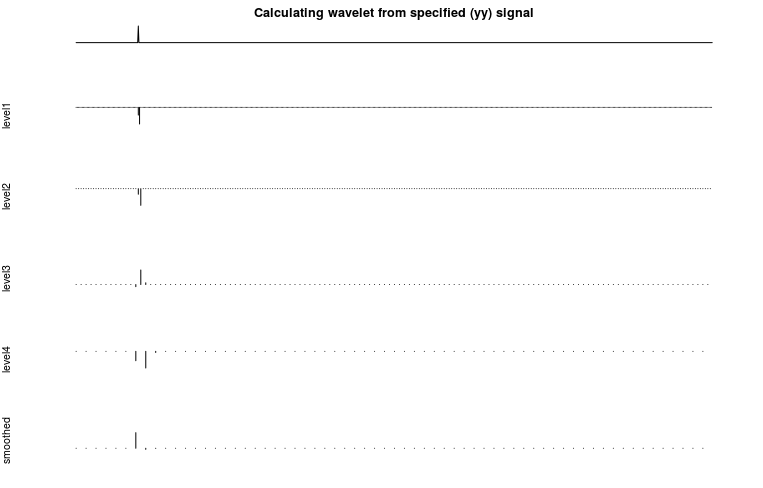
\includegraphics[scale=0.55]{processed-signal.png}
\caption{Presented plots are in steps of shown calculation}
\label{fig:plotting-fig}
\end{figure}



\subsection{Wavelet calculation details}

To complete our discussion of the Discrete Wavelet Transform (DWT), let’s look at how the wavelet coefficient matrix is
applied to the data vector. The matrix is applied in a hierarchical algorithm, sometimes called \textit{a
pyramidal algorithm}. The wavelet coefficients are arranged so that odd rows contain an ordering of
wavelet coefficients that act as the smoothing filter, and the even rows contain an ordering of wavelet
coefficient with different signs that act to bring out the data’s detail. The matrix is first applied to
the original, full-length vector. Then the vector is smoothed and decimated by half and the matrix
is applied again. Then the smoothed, halved vector is smoothed, and halved again, and the matrix
applied once more. This process continues until a trivial number of “smooth-smooth-smooth...”
data remain. That is, each matrix application brings out a higher resolution of the data while at
the same time smoothing the remaining data. The output of the DWT consists of the remaining
“smooth (etc.)” components, and all of the accumulated “detail” components.

The DWT matrix is not sparse in general, so we face the same complexity issues that we had
previously faced for the discrete Fourier transform \cite{wickerhauser1994adapted}. We solve it as we did for the Fast Fourier transform (FFT), by
factoring the DWT into a product of a few sparse matrices using self-similarity properties. The
result is an algorithm that requires only order n operations to transform an n-sample vector. This
is the “fast” DWT of Mallat and Daubechies.


\section{Signal Examples}

\begin{figure}[h!]
\begin{lstlisting}
data(ibm)     
yy <- diff(log(ibm))
\end{lstlisting}

\caption{Datasource from \cite{genccay2001introduction}}
\end{figure}

\begin{figure}[h!]
\begin{lstlisting}
x = 1:1024
yy = ifelse(x <= 100, 0, ifelse(x < 600, 1, 0))
\end{lstlisting}
\caption{Same values in wider interval}
\end{figure}

\begin{figure}[h!]
\begin{lstlisting}
x = 1:1024
yy = runif(1024, -1.0, 1.0)
\end{lstlisting}
\caption{Randomized values}
\end{figure}

\begin{figure}[h!]
\begin{lstlisting}
x = 1:1024
yy = DJ.EX()$doppler;
\end{lstlisting}
\caption{Doppler signal}
\end{figure}


\bibliographystyle{plain}
\bibliography{references}
\end{document}
